% Preambolo comune al libro completo (main.tex) e ai volumi autonomi (libro-*.tex).
\usepackage[margin=1in]{geometry}
%\usepackage[italian]{babel}, \usepackage[T1]{fontenc},
\usepackage[utf8]{inputenc} \usepackage{booktabs}
\usepackage{amsmath, amsfonts}
\usepackage{graphicx}
\usepackage{enumitem, url, siunitx, comment, booktabs}
\usepackage[colorlinks=true, linkcolor=blue]{hyperref}

\usepackage{amssymb, amsthm, algpseudocode}
\usepackage{bm}
\usepackage{mathtools}
\usepackage{tikz}
\usetikzlibrary{shapes.geometric,shapes.symbols,shapes.misc, arrows.meta,positioning,calc,fit}

\newtheorem{theorem}{Theorem}[chapter]
\newtheorem{definition}{Definition}[chapter]
\newtheorem{remark}{Remark}[chapter]
\newtheorem{example}{Example}[chapter]
\newtheorem{question}{Question}[chapter]


% Indice: spazio piu' largo per i numeri lunghi (es. 0.9.10, 2.1.10.3)
\usepackage{etoolbox}
\makeatletter
\patchcmd{\l@chapter}{1.5em}{2.4em}{}{}
\renewcommand*\l@section{\@dottedtocline{1}{1.5em}{3.3em}}
\renewcommand*\l@subsection{\@dottedtocline{2}{4.8em}{4.3em}}
\makeatother

% ---------------------------------------------------------------------
% Figure: le immagini tratte dalle slide e dalle dispense delle lezioni
% ---------------------------------------------------------------------
\usepackage{morefloats}
\extrafloats{150}
\setcounter{topnumber}{3}
\setcounter{bottomnumber}{2}
\setcounter{totalnumber}{5}
\renewcommand{\topfraction}{0.85}
\renewcommand{\bottomfraction}{0.6}
\renewcommand{\textfraction}{0.12}
\renewcommand{\floatpagefraction}{0.7}

% \slidefig{file}{didascalia}{fonte}{etichetta}
% Inserisce una slide (o un collage di slide) con didascalia e fonte.
\newcommand{\slidefig}[4]{%
  \begin{figure}[htbp]
    \centering
    \includegraphics[width=0.92\textwidth,height=0.42\textheight,keepaspectratio]{#1}
    \caption[#2]{#2 {\footnotesize\textit{(Fonte: #3.)}}}%
    \label{#4}
  \end{figure}}

% ---------------------------------------------------------------------
% Copertine dei volumi e delle parti
% ---------------------------------------------------------------------
% =====================================================================
%  copertine.tex -- copertine dei volumi e illustrazioni delle parti
% ---------------------------------------------------------------------
%  Uso:
%    \copertinaLibro{<chiave>}            copertina a tutta pagina di un volume
%    \parteillustrata{<chiave>}{<titolo>}  \part{<titolo>} con la pagina illustrata
%  Chiavi: completo, seminari, conferenze, unreal, agd, professioni,
%          gamedesign, revisioni.
%  Ogni copertina e' disegnata in TikZ (con alcune fotografie tratte dalle
%  slide delle lezioni per AGD e Game Design). La parte centrale resta
%  libera: nei volumi ospita titolo e autore, nel libro completo ospita il
%  titolo della parte stampato da \part.
% =====================================================================
\usetikzlibrary{shadows,decorations.pathmorphing,decorations.markings}

% --- Palette ----------------------------------------------------------
\definecolor{copNavy}{HTML}{0F1B33}
\definecolor{copGold}{HTML}{E8B84A}
\definecolor{copOrange}{HTML}{F08A24}
\definecolor{copRed}{HTML}{B5292E}
\definecolor{copPurple}{HTML}{241238}
\definecolor{copViolet}{HTML}{7B3FA0}
\definecolor{copBlueprint}{HTML}{1C2838}
\definecolor{copGridA}{HTML}{26364A}
\definecolor{copGridB}{HTML}{33485F}
\definecolor{copFelt}{HTML}{1E5C3C}
\definecolor{copFeltDark}{HTML}{123D27}
\definecolor{copTeal}{HTML}{0E4D55}
\definecolor{copTealLight}{HTML}{4FB3BF}
\definecolor{copSlate}{HTML}{22262E}
\definecolor{copCyan}{HTML}{3FC1E0}
\definecolor{copPaper}{HTML}{FBF8EF}
\definecolor{copRule}{HTML}{BFD3E6}
\definecolor{copPen}{HTML}{D0262B}
\definecolor{copPostit}{HTML}{FFE873}

% --- Elementi grafici riutilizzabili -----------------------------------
\tikzset{
  % dado a sei facce: faccia del 5
  dado5/.pic={
    \draw[pic actions, rounded corners=2.5pt, line width=0.6pt] (-.5,-.5) rectangle (.5,.5);
    \foreach \p in {(-.24,-.24),(.24,.24),(-.24,.24),(.24,-.24),(0,0)}
      \fill[black!85] \p circle (.085);
  },
  % dado a sei facce: faccia del 3
  dado3/.pic={
    \draw[pic actions, rounded corners=2.5pt, line width=0.6pt] (-.5,-.5) rectangle (.5,.5);
    \foreach \p in {(-.24,-.24),(.24,.24),(0,0)}
      \fill[black!85] \p circle (.085);
  },
  % meeple stilizzato
  meeple/.pic={
    \fill[pic actions] (0,.78) circle (.2);
    \fill[pic actions] (-.48,0) -- (-.14,0) -- (0,.24) -- (.14,0) -- (.48,0)
      -- (.22,.36) -- (.56,.5) to[out=90,in=0] (.3,.62) -- (-.3,.62)
      to[out=180,in=90] (-.56,.5) -- (-.22,.36) -- cycle;
  },
  % carta da gioco
  carta/.pic={
    \draw[pic actions, rounded corners=3pt, line width=0.6pt] (-.7,-1) rectangle (.7,1);
    \draw[rounded corners=2pt, line width=0.4pt, black!30] (-.55,-.85) rectangle (.55,.85);
  },
  % controller
  pad/.pic={
    \fill[pic actions, rounded corners=10pt] (-1.9,-.55) rectangle (1.9,.85);
    \fill[pic actions] (-1.45,-.45) circle (.8);
    \fill[pic actions] (1.45,-.45) circle (.8);
    \fill[copNavy] (-1.55,.05) rectangle (-1.05,.25);
    \fill[copNavy] (-1.4,-.1) rectangle (-1.2,.4);
    \foreach \p in {(1.3,.15),(1.55,.4),(1.55,-.1),(1.8,.15)}
      \fill[copNavy] \p circle (.1);
  },
  % cubo isometrico (blockout)
  cubo/.pic={
    \fill[pic actions, fill=black!55] (0,0) -- (.87,.5) -- (.87,1.5) -- (0,1) -- cycle;
    \fill[pic actions, fill=black!35] (0,0) -- (-.87,.5) -- (-.87,1.5) -- (0,1) -- cycle;
    \fill[pic actions, fill=black!15] (0,1) -- (.87,1.5) -- (0,2) -- (-.87,1.5) -- cycle;
  },
  % fumetto
  fumetto/.style={rounded corners=8pt, fill=white, fill opacity=.92, text opacity=1,
    inner xsep=10pt, inner ysep=7pt, font=\sffamily\bfseries},
  % fotografia con bordo bianco (polaroid)
  polaroid/.style={fill=white, inner sep=5pt, inner ysep=5pt, drop shadow={opacity=.45}},
}

% Nodo Blueprint: \copBPnode{x}{y}{larghezza}{colore}{titolo}{righe}
\newcommand{\copBPnode}[6]{%
  \begin{scope}[shift={(#1,#2)}]
    \fill[black, opacity=.35, rounded corners=4pt] (.12,-.12) rectangle ++(#3,-#6*0.55-.9);
    \fill[black!80, fill opacity=.92, rounded corners=4pt] (0,0) rectangle ++(#3,-#6*0.55-.9);
    \fill[#4, rounded corners=4pt] (0,0) rectangle ++(#3,-.7);
    \fill[#4] (0,-.4) rectangle ++(#3,-.3);
    \node[anchor=west, text=white, font=\sffamily\bfseries\small] at (.2,-.35) {#5};
    \foreach \r in {1,...,#6} {
      \fill[white!85!black] (.3,-.55-\r*0.55) circle (.09);
      \fill[white!30!black] (.55,-.6-\r*0.55) rectangle ++(1.3,.12);
    }
    \fill[white] (.15,-1.0) -- (.32,-1.0) -- (.42,-1.1) -- (.32,-1.2) -- (.15,-1.2) -- cycle;
    \fill[white] (#3-.45,-1.0) -- (#3-.28,-1.0) -- (#3-.18,-1.1) -- (#3-.28,-1.2) -- (#3-.45,-1.2) -- cycle;
  \end{scope}}

% --- Dati dei volumi -----------------------------------------------------
\makeatletter
\def\copertina@titolo@completo{La Bibbia del Game Design}
\def\copertina@sotto@completo{Lezioni, seminari e conferenze: il libro completo}
\def\copertina@vol@completo{Edizione completa}
\def\copertina@col@completo{copNavy}

\def\copertina@titolo@seminari{Seminari per il Game Designer}
\def\copertina@sotto@seminari{Feedback, leadership, Agile, producer, mindset, audio}
\def\copertina@vol@seminari{Volume 0}
\def\copertina@col@seminari{copRed}

\def\copertina@titolo@conferenze{Conferenze}
\def\copertina@sotto@conferenze{GAMM di Roma -- Checkpoint Festival \textperiodcentered\ On The Road, Zagarolo}
\def\copertina@vol@conferenze{Volume C}
\def\copertina@col@conferenze{copViolet}

\def\copertina@titolo@unreal{Fondamenti di Unreal Engine}
\def\copertina@sotto@unreal{Blueprint, materiali, animazione, luci e livelli}
\def\copertina@vol@unreal{Volume 1}
\def\copertina@col@unreal{copBlueprint}

\def\copertina@titolo@agd{Analog Game Design}
\def\copertina@sotto@agd{Giochi da tavolo, di ruolo, LARP e giochi pervasivi}
\def\copertina@vol@agd{Volume 2}
\def\copertina@col@agd{copFeltDark}

\def\copertina@titolo@professioni{Alcune Professioni nel Mondo Videoludico}
\def\copertina@sotto@professioni{Game, level e narrative design, animazione, programmazione, 3D art}
\def\copertina@vol@professioni{Volume 3}
\def\copertina@col@professioni{copTeal}

\def\copertina@titolo@gamedesign{Game Design}
\def\copertina@sotto@gamedesign{Metodi di design, documentazione e level design}
\def\copertina@vol@gamedesign{Volume 4}
\def\copertina@col@gamedesign{copSlate}

\def\copertina@titolo@revisioni{Revisioni dei Compiti}
\def\copertina@sotto@revisioni{Gli errori ricorrenti nei task, e come evitarli}
\def\copertina@vol@revisioni{Volume 5}
\def\copertina@col@revisioni{copPen}

% --- Sfondi ---------------------------------------------------------------
% Ogni sfondo disegna in coordinate di pagina (cm), con \W e \H dimensioni
% del foglio. La fascia centrale (circa H/2 +- 4.6 cm) resta per i testi.

% Libro completo: tavolo da gioco notturno, analogico e digitale insieme
\def\copertina@completo{%
  \fill[copNavy] (0,0) rectangle (\W,\H);
  \begin{scope}[opacity=.13]
    \foreach \i in {0,...,14} \foreach \j in {0,...,20} {
      \pgfmathsetmacro{\hx}{\i*1.6 + mod(\j,2)*0.8}
      \pgfmathsetmacro{\hy}{\j*1.39}
      \node[draw=copGold, line width=.5pt, regular polygon, regular polygon sides=6,
            minimum size=1.6cm, inner sep=0pt] at (\hx,\hy) {};
    }
  \end{scope}
  % alone centrale
  \fill[copGold, opacity=.06] (\W/2,\H/2) circle (10);
  % icone in alto
  \pic[fill=copGold, rotate=-12, scale=1.6] at (3.4,\H-4.4) {dado5};
  \pic[fill=white, rotate=18, scale=1.1] at (5.4,\H-3.1) {dado3};
  \pic[fill=copGold, scale=1.15] at (\W-4,\H-4.6) {pad};
  \pic[fill=copRed, scale=1.3] at (\W/2-1.2,\H-5.2) {meeple};
  \pic[fill=copCyan, scale=1.3] at (\W/2+1.2,\H-5.2) {meeple};
  \pic[fill=white, rotate=-8] at (\W/2-3.6,\H-3) {carta};
  \pic[fill=copGold!30, rotate=6] at (\W/2+3.4,\H-2.8) {carta};
  % mini flowchart in basso
  \begin{scope}[shift={(2.2,4.6)}, every node/.style={font=\sffamily\scriptsize\bfseries, text=copNavy}]
    \node[fill=copGold, rounded corners=6pt, minimum width=1.6cm, minimum height=.7cm] (a) at (0,0) {START};
    \node[fill=white, minimum width=1.8cm, minimum height=.7cm] (b) at (3,0) {IDEA};
    \node[fill=copCyan, diamond, aspect=1.6, inner sep=1pt] (c) at (6.3,0) {PLAYTEST?};
    \node[fill=white, minimum width=1.8cm, minimum height=.7cm] (d) at (9.8,0) {ITERA};
    \node[fill=copGold, rounded corners=6pt, minimum width=1.6cm, minimum height=.7cm] (e) at (13.4,0) {GIOCO};
    \draw[-{Stealth[length=3mm]}, white, line width=1pt] (a) -- (b);
    \draw[-{Stealth[length=3mm]}, white, line width=1pt] (b) -- (c);
    \draw[-{Stealth[length=3mm]}, white, line width=1pt] (c) -- (d);
    \draw[-{Stealth[length=3mm]}, white, line width=1pt] (d) -- (e);
    \draw[-{Stealth[length=3mm]}, white, line width=1pt, dashed] (d.south) to[bend left=35] (b.south);
  \end{scope}
  % dorsi dei sette volumi
  \foreach \c/\t [count=\k] in {copRed/0, copViolet/C, copBlueprint/1, copFelt/2, copTeal/3, copSlate/4, copPen/5} {
    \pgfmathsetmacro{\sx}{\W/2 - 7*1.1/2 + (\k-1)*1.1}
    \fill[\c, draw=copGold, line width=.6pt] (\sx,1.2) rectangle ++(1,2.2);
    \node[text=copGold, font=\sffamily\bfseries] at (\sx+.5,2.3) {\t};
  }
}

% Seminari: un caldo dialogo di fumetti
\def\copertina@seminari{%
  \shade[top color=copOrange, bottom color=copRed] (0,0) rectangle (\W,\H);
  \foreach \x/\y/\r in {3/24/2.4, 18/22.5/3.2, 9/26/1.4, 19/5/2.6, 2.5/4/1.8, 11/2/1.1}
    \fill[white, opacity=.08] (\x,\y) circle (\r);
  \foreach \x/\y/\t/\a in {
      2.6/\H-2.6/Feedback/-6, 9.0/\H-2.0/Leadership/4, 15.6/\H-2.9/Agile e Scrum/-3,
      4.8/\H-5.3/Publisher/5, 11.3/\H-4.9/Producer/-4, 17.2/\H-5.9/Mindset/7,
      3.4/5.4/Hackerare un gioco/4, 11.0/6.0/Metaverso/-5, 17.0/4.8/Game audio/3,
      6.8/2.4/Tempo e idee/-3, 14.8/2.1/Cultura del feedback/2} {
    \node[fumetto, text=copRed, rotate=\a, font=\sffamily\bfseries\large] (f) at (\x,\y) {\t};
    \fill[white, opacity=.92, rotate around={\a:(f.center)}]
      ([xshift=-6pt]f.south) -- ([xshift=6pt]f.south) -- ([xshift=-14pt,yshift=-10pt]f.south) -- cycle;
  }
  % microfono
  \begin{scope}[shift={(\W-2.4,\H/2+5.4)}, rotate=-20]
    \fill[white, opacity=.9, rounded corners=8pt] (-.45,0) rectangle (.45,1.4);
    \fill[copRed!70!black] (-.12,-1.6) rectangle (.12,0);
    \draw[white, line width=1.5pt] (-.65,.6) to[out=-90,in=-90] (.65,.6);
  \end{scope}
}

% Conferenze: palco, riflettori e pubblico
\def\copertina@conferenze{%
  \fill[copPurple] (0,0) rectangle (\W,\H);
  % riflettori
  \foreach \x/\tx in {3/6, .5*\W/.5*\W, \W-3/\W-6} {
    \fill[white, opacity=.10] (\x,\H) -- (\tx-3.2,3.2) -- (\tx+3.2,3.2) -- cycle;
    \fill[copGold] (\x,\H-.1) circle (.35);
  }
  % sipario
  \foreach \s/\d in {0/1, \W/-1} {
    \foreach \k in {0,...,4}
      \fill[copRed!80!black, opacity=.9]
        ({\s+\d*\k*0.35},\H) .. controls ({\s+\d*(\k*0.35+0.6)},{\H/2}) .. ({\s+\d*\k*0.25},2.5)
        -- (\s,2.5) -- (\s,\H) -- cycle;
  }
  \fill[copRed!70!black] (0,\H-1.2) -- (\W,\H-1.2) -- (\W,\H) -- (0,\H) -- cycle;
  \foreach \k in {0,...,11}
    \fill[copRed!55!black] (\k*\W/12,\H-1.2) arc (180:360:\W/24 and .45);
  % palco
  \fill[copViolet!45!black] (0,2.5) rectangle (\W,3.6);
  \foreach \x/\y in {6/3.2, \W/2/3.2, \W-6/3.2} \fill[white, opacity=.15] (\x,\y) ellipse (3.2 and .35);
  % leggio
  \fill[copGold!80!black] (\W/2-.8,3.6) -- (\W/2+.8,3.6) -- (\W/2+.5,5.3) -- (\W/2-.5,5.3) -- cycle;
  % pubblico
  \foreach \k in {0,...,13} {
    \pgfmathsetmacro{\px}{0.8+\k*1.55}
    \fill[black] (\px,1.6) circle (.42);
    \fill[black] (\px-.75,0) .. controls (\px-.75,1.2) and (\px+.75,1.2) .. (\px+.75,0) -- cycle;
  }
  % badge degli eventi
  \node[fill=copGold, text=copPurple, rounded corners=4pt, font=\sffamily\bfseries\small, rotate=-4]
    at (5.2,\H-3.4) {GAMM -- Checkpoint Festival, Roma};
  \node[fill=white, text=copPurple, rounded corners=4pt, font=\sffamily\bfseries\small, rotate=3]
    at (\W-5.6,\H-4.4) {On The Road -- Zagarolo};
}

% Unreal Engine: la griglia dei Blueprint
\def\copertina@unreal{%
  \fill[copBlueprint] (0,0) rectangle (\W,\H);
  \draw[copGridA, line width=.3pt, step=.5] (0,0) grid (\W,\H);
  \draw[copGridB, line width=.7pt, step=2.5] (0,0) grid (\W,\H);
  % nodi in alto
  \copBPnode{1.3}{\H-1.6}{4.4}{copRed}{Event BeginPlay}{1}
  \copBPnode{8.2}{\H-2.6}{5.4}{blue!55!black}{Spawn Actor from Class}{3}
  \copBPnode{15.0}{\H-1.4}{5.0}{blue!55!black}{Set Timer by Event}{2}
  % nodi in basso
  \copBPnode{1.6}{7.6}{4.0}{gray!60!black}{Branch}{2}
  \copBPnode{8.0}{6.6}{5.0}{green!45!black}{Get Player Character}{1}
  \copBPnode{14.6}{7.9}{4.4}{blue!55!black}{Print String}{2}
  % fili di esecuzione e dati
  \draw[white, line width=1.6pt] (5.5,\H-2.7) .. controls (7,\H-2.7) and (6.8,\H-3.7) .. (8.3,\H-3.7);
  \draw[white, line width=1.6pt] (13.4,\H-3.7) .. controls (14.6,\H-3.7) and (13.8,\H-2.5) .. (15.1,\H-2.5);
  \draw[copCyan, line width=1.4pt] (13.4,\H-4.9) .. controls (16,\H-4.9) and (15,\H-3.6) .. (15.3,\H-3.6);
  \draw[white, line width=1.6pt] (5.4,6.5) .. controls (6.8,6.5) and (6.6,5.5) .. (8.1,5.5);
  \draw[copRed!60, line width=1.4pt] (13.0,5.0) .. controls (14,5.0) and (13.6,6.4) .. (14.8,6.4);
  \draw[white, line width=1.6pt] (12.8,5.5) .. controls (14.0,5.5) and (13.6,6.8) .. (14.7,6.8);
  % cubo di Unreal (wireframe)
  \begin{scope}[shift={(\W/2,1.6)}, scale=.9, copCyan, line width=1pt]
    \draw (0,0) -- (1.6,.9) -- (1.6,2.7) -- (0,1.8) -- cycle;
    \draw (0,0) -- (-1.6,.9) -- (-1.6,2.7) -- (0,1.8);
    \draw (-1.6,2.7) -- (0,3.6) -- (1.6,2.7);
  \end{scope}
}

% Analog Game Design: il tavolo da gioco, con le foto delle lezioni
\def\copertina@agd{%
  \fill[copFelt] (0,0) rectangle (\W,\H);
  \shade[inner color=copFelt!70!white, outer color=copFelt, opacity=.6] (\W/2,\H/2) circle (12);
  % tessere esagonali
  \foreach \i/\j/\c in {0/0/brown!70, 1/0/green!50!black, 2/0/yellow!70!brown, 0/1/blue!40!gray,
                        1/1/brown!50, 2/1/green!35!black, 3/0/orange!70!brown, 3/1/gray!60} {
    \pgfmathsetmacro{\hx}{1.4 + \i*1.75 + mod(\j,2)*0.875}
    \pgfmathsetmacro{\hy}{1.3 + \j*1.52}
    \node[fill=\c, draw=copFeltDark, line width=1.2pt, regular polygon, regular polygon sides=6,
          minimum size=2cm, inner sep=0pt] at (\hx,\hy) {};
  }
  % carte a ventaglio
  \foreach \a/\c in {-24/copRed!80, -8/copGold, 8/white, 24/copCyan!70} \pic[fill=\c, rotate=\a, scale=1.25] at (\W-3.2,2.2) {carta};
  % dadi e meeple
  \pic[fill=white, rotate=14, scale=.9] at (10.2,1.7) {dado5};
  \pic[fill=copRed!80, rotate=-20, scale=.9] at (11.6,2.4) {dado3};
  \pic[fill=copGold, scale=1.1] at (13.6,1.4) {meeple};
  \pic[fill=copCyan, scale=1.1] at (8.6,1.6) {meeple};
  \pic[fill=white, scale=.8] at (\W-1.3,\H-1.6) {meeple};
  \pic[fill=copRed!80, scale=.8] at (1.2,\H-1.5) {meeple};
  % fotografie dalle lezioni
  \node[polaroid, rotate=-7]  at (4.3,\H-4.6)  {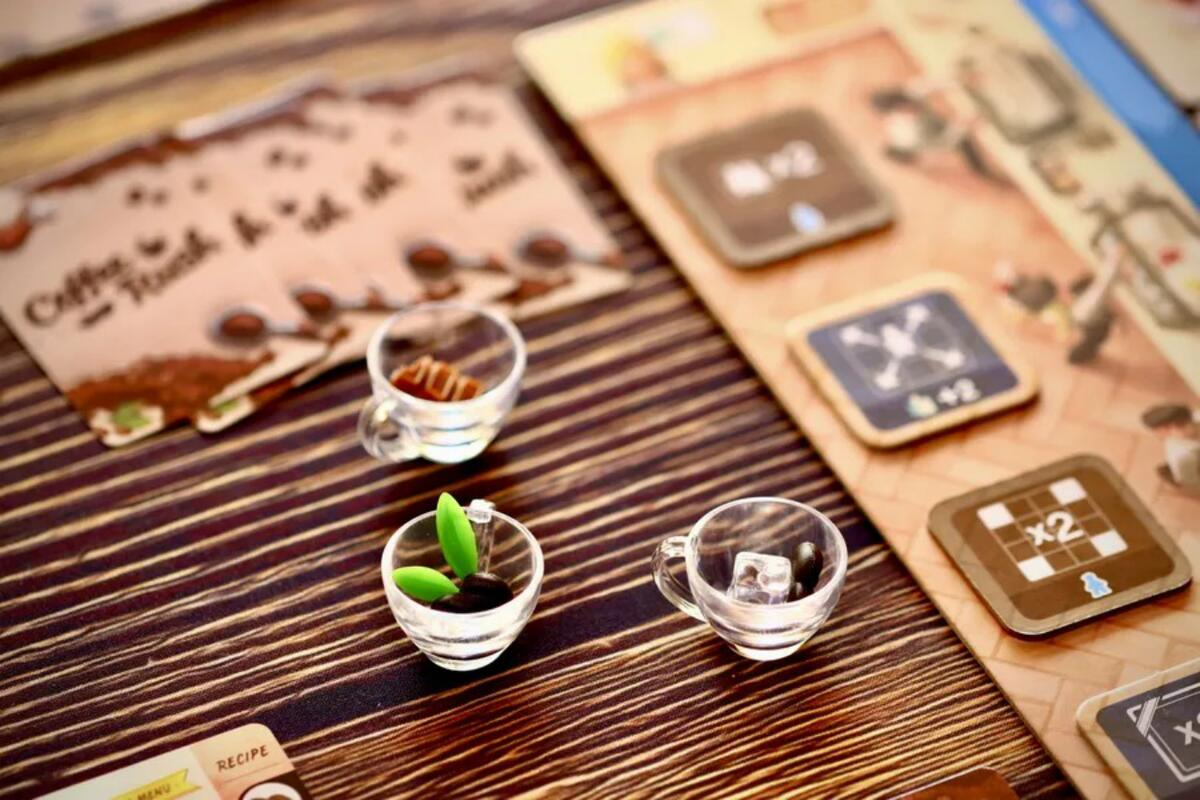
\includegraphics[width=5.2cm]{img/copertine/agd-coffee}};
  \node[polaroid, rotate=5]   at (\W/2+.2,\H-3.6) {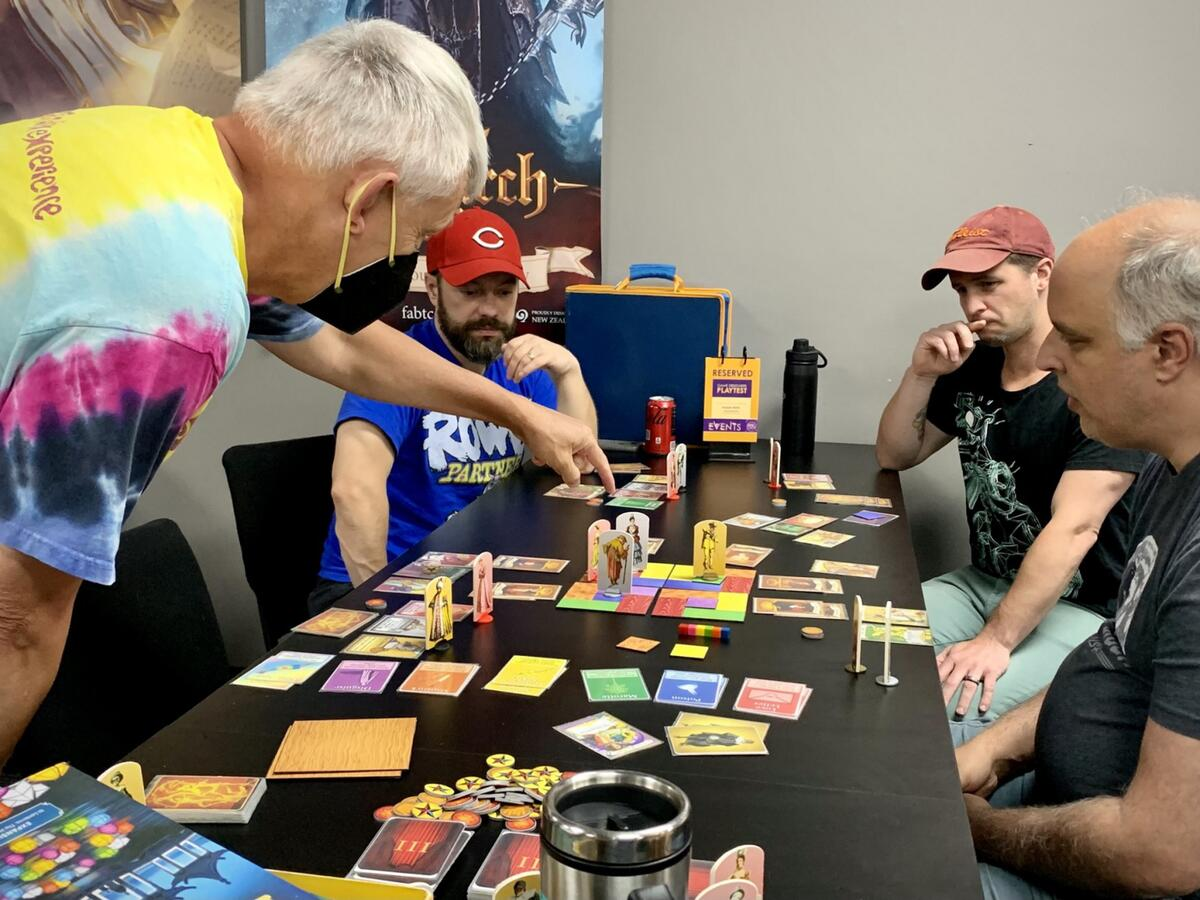
\includegraphics[width=4.6cm]{img/copertine/agd-playtest}};
  \node[polaroid, rotate=-3]  at (\W-4.2,\H-4.9) {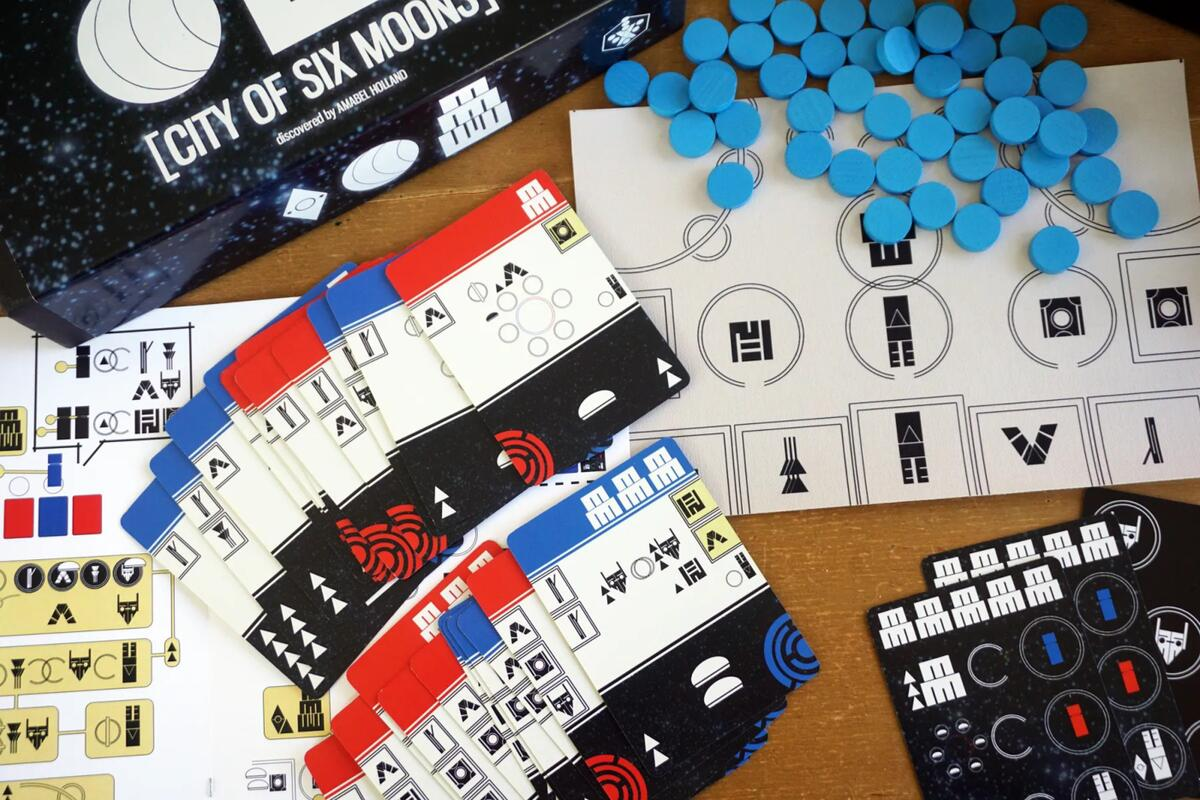
\includegraphics[width=5.0cm]{img/copertine/agd-city}};
  \node[polaroid, rotate=6]   at (3.8,7.9)  {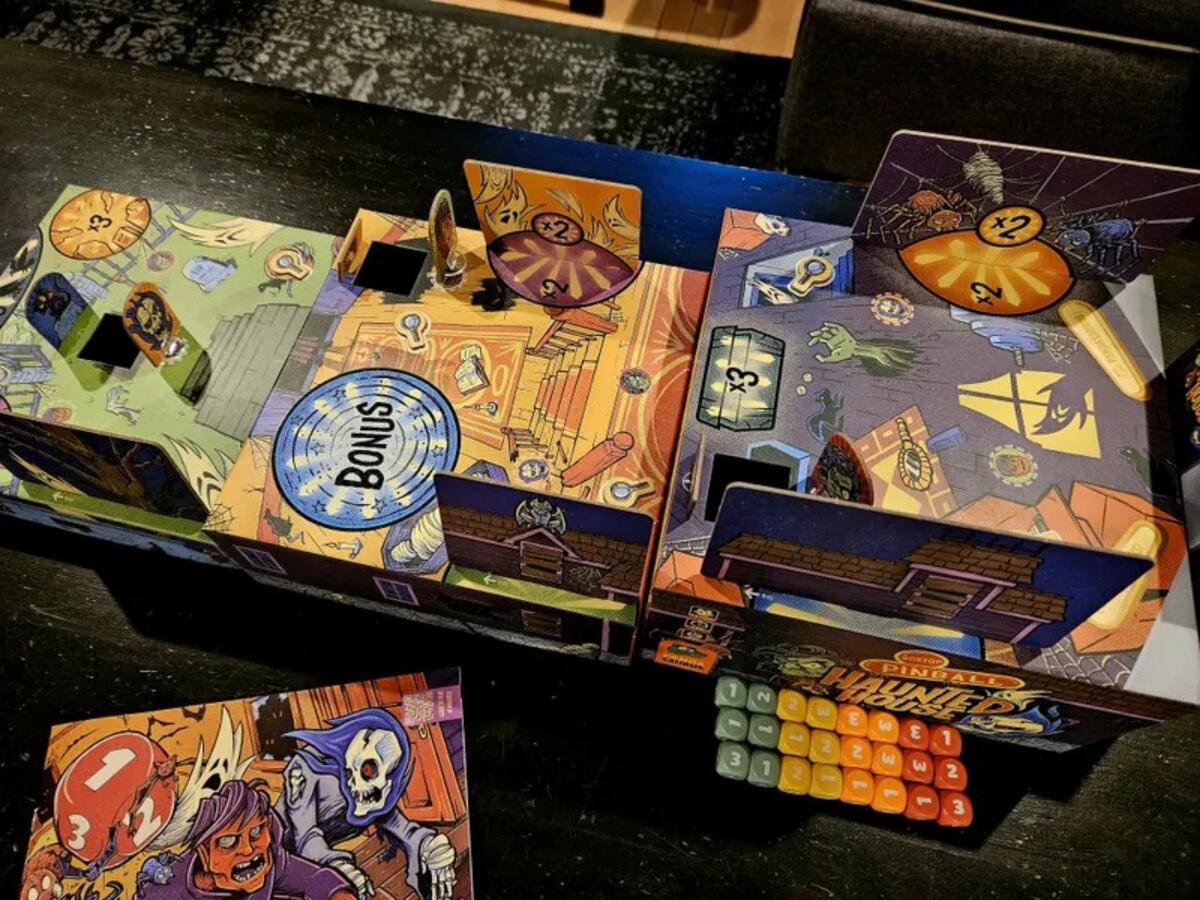
\includegraphics[width=4.8cm]{img/copertine/agd-pinball}};
  \node[polaroid, rotate=-4]  at (\W/2+.4,7.2) {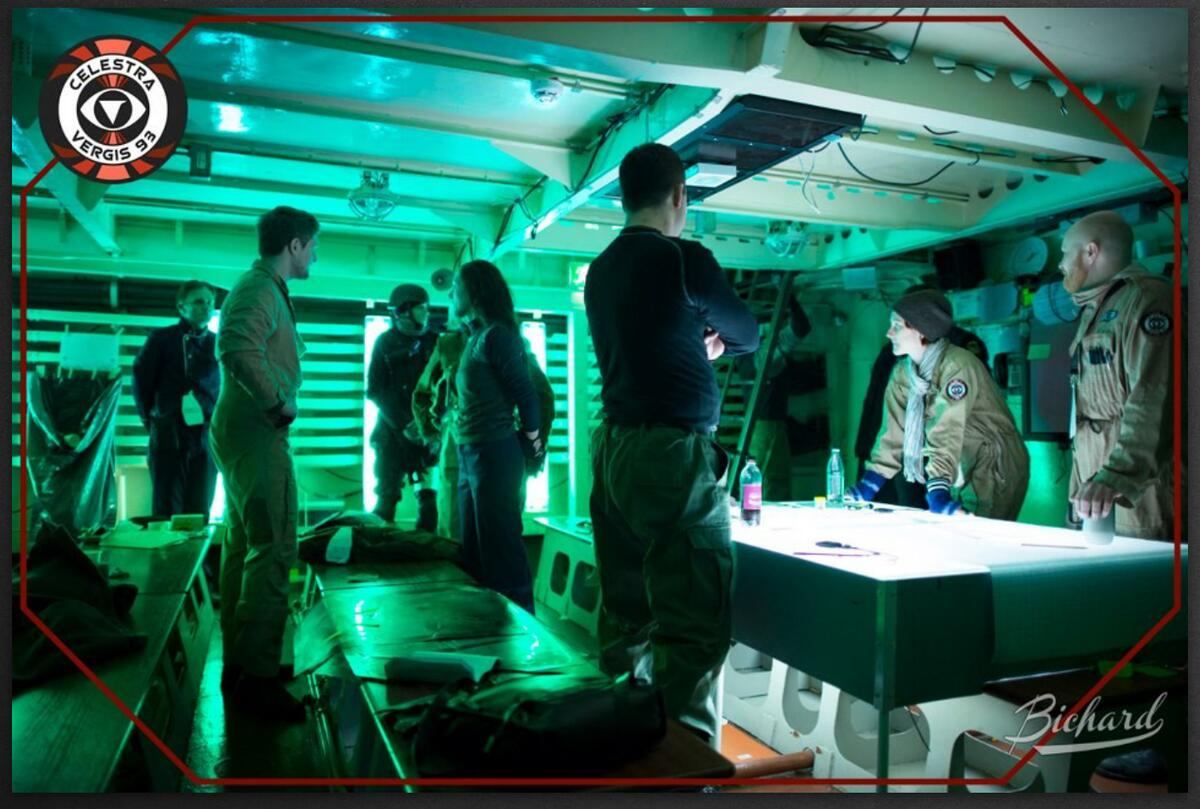
\includegraphics[width=4.6cm]{img/copertine/agd-larp}};
  \node[polaroid, rotate=4]   at (\W-4.0,7.8)  {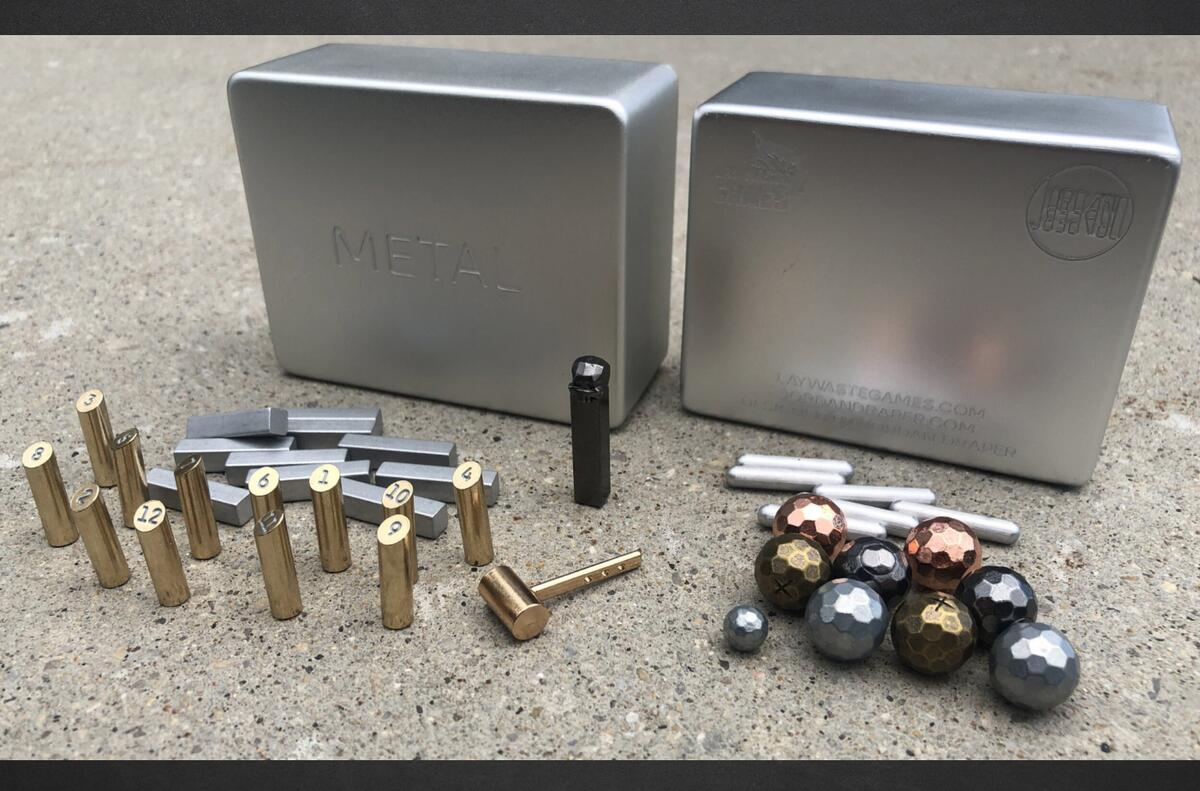
\includegraphics[width=4.8cm]{img/copertine/agd-metal}};
}

% Professioni: la rete dei mestieri
\def\copertina@professioni{%
  \fill[copTeal] (0,0) rectangle (\W,\H);
  \foreach \k in {1,...,9} \draw[copTealLight, opacity=.12, line width=.8pt] (\W/2,\H/2) circle (\k*1.6);
  \foreach \x/\y/\t/\i [count=\n] in {
      3.6/\H-3.6/Game designer/d, .5*\W/\H-2.6/Level designer/l, \W-3.6/\H-3.6/Narrative designer/n,
      3.6/4.4/Character animator/a, .5*\W/3.4/Programmatore/p, \W-3.6/4.4/3D artist/c} {
    \draw[copTealLight, line width=1.2pt, opacity=.6] (\x,\y) -- (.5*\W,.5*\H);
    \fill[white] (\x,\y) circle (1.35);
    \fill[copTealLight] (\x,\y) circle (1.15);
    \node[text=white, font=\sffamily\bfseries\small, below] at (\x,\y-1.45) {\t};
    \begin{scope}[shift={(\x,\y)}]
      \ifnum\n=1 \pic[fill=white, scale=.95, rotate=10] at (0,0) {dado5}; \fi
      \ifnum\n=2 \pic[scale=.55] at (0,-.6) {cubo}; \fi
      \ifnum\n=3 \node[fill=white, rounded corners=5pt, text=copTeal, font=\bfseries\Large, inner sep=4pt] at (0,0) {``\,\dots''}; \fi
      \ifnum\n=4 \begin{scope}[white, line width=2pt, line cap=round]
                 \fill (0,.55) circle (.2); \draw (0,.35) -- (0,-.2) -- (-.35,-.65); \draw (0,-.2) -- (.4,-.6);
                 \draw (-.45,.25) -- (0,.15) -- (.45,.4); \end{scope} \fi
      \ifnum\n=5 \node[text=white, font=\ttfamily\bfseries\LARGE] at (0,0) {\{\,\}}; \fi
      \ifnum\n=6 \begin{scope}[white, line width=1.4pt, scale=.55]
                 \draw (0,-1) -- (.87,-.5) -- (.87,.5) -- (0,0) -- cycle; \draw (0,-1) -- (-.87,-.5) -- (-.87,.5) -- (0,0);
                 \draw (-.87,.5) -- (0,1) -- (.87,.5); \end{scope} \fi
    \end{scope}
  }
}

% Game Design: flowchart, blockout e un rullino di immagini
\def\copertina@gamedesign{%
  \fill[copSlate] (0,0) rectangle (\W,\H);
  \draw[white, opacity=.05, step=1] (0,0) grid (\W,\H);
  % flowchart in alto
  \begin{scope}[shift={(0,\H-3.3)}, every node/.style={font=\sffamily\bfseries\small, text=copSlate}]
    \node[fill=copCyan, rounded corners=8pt, minimum width=2.2cm, minimum height=.9cm] (s) at (2.6,0) {Start};
    \node[fill=white, minimum width=2.6cm, minimum height=.9cm] (r) at (6.8,0) {Ricerca};
    \node[fill=copGold, diamond, aspect=1.7, inner sep=1.5pt] (d) at (11.2,0) {Funziona?};
    \node[fill=white, minimum width=2.4cm, minimum height=.9cm] (i) at (11.2,-2.2) {Itera};
    \node[fill=copCyan, rounded corners=8pt, minimum width=2.2cm, minimum height=.9cm] (e) at (15.8,0) {Vision};
    \draw[-{Stealth[length=3mm]}, white, line width=1.1pt] (s) -- (r);
    \draw[-{Stealth[length=3mm]}, white, line width=1.1pt] (r) -- (d);
    \draw[-{Stealth[length=3mm]}, white, line width=1.1pt] (d) -- node[above, text=white, font=\sffamily\scriptsize] {s\`i} (e);
    \draw[-{Stealth[length=3mm]}, white, line width=1.1pt] (d) -- node[right, text=white, font=\sffamily\scriptsize] {no} (i);
    \draw[-{Stealth[length=3mm]}, white, line width=1.1pt] (i) -| (r);
  \end{scope}
  % blockout isometrico ai lati
  \foreach \x/\y/\s in {1.6/.5*\H+5.6/.8, 2.6/.5*\H+5.1/.55, \W-1.8/.5*\H+5.4/.9, \W-2.9/.5*\H+5.0/.5}
    \pic[scale=\s] at (\x,\y) {cubo};
  % rullino
  \fill[black] (0,1.0) rectangle (\W,6.4);
  \foreach \k in {0,...,26} {
    \fill[copSlate!40] (.3+\k*.8,1.2) rectangle ++(.45,.3);
    \fill[copSlate!40] (.3+\k*.8,5.9) rectangle ++(.45,.3);
  }
  \foreach \f/\x in {gd-blockout/2.9, gd-uncharted/8.2, gd-interior/13.5, gd-liesofp/18.6}
    \node[inner sep=0pt] at (\x,3.7) {\includegraphics[height=3.9cm,width=4.9cm,keepaspectratio]{img/copertine/\f}};
}

% Revisioni: un foglio corretto a penna rossa
\def\copertina@revisioni{%
  \fill[copPaper] (0,0) rectangle (\W,\H);
  \foreach \k in {1,...,34} \draw[copRule, line width=.5pt] (0,\k*0.8) -- (\W,\k*0.8);
  \draw[copPen!70, line width=.8pt] (2.6,0) -- (2.6,\H);
  % righe di testo stilizzate in alto e in basso
  \foreach \y/\l in {\H-2.0/14, \H-2.8/16.5, \H-3.6/12, \H-4.4/15.5, \H-5.2/9,
                     6.4/15, 5.6/13, 4.8/16, 4.0/11, 3.2/14.5, 2.4/8} {
    \fill[black!45, rounded corners=1pt] (3.2,\y-.12) rectangle ++(\l,.24);
  }
  % correzioni
  \draw[copPen, line width=1.6pt, decorate, decoration={zigzag, amplitude=1.2pt, segment length=4pt}]
    (6,\H-2.8) -- (13.5,\H-2.8);
  \draw[copPen, line width=1.4pt] (10.6,\H-4.4) ellipse (2.8 and .45);
  \draw[copPen, line width=1.6pt, decorate, decoration={zigzag, amplitude=1.2pt, segment length=4pt}]
    (4.5,4.8) -- (12.5,4.8);
  \draw[copPen, line width=1.4pt] (8.8,2.4) ellipse (3 and .45);
  \node[text=copPen, font=\sffamily\bfseries\Huge, rotate=8] at (1.3,\H-3.6) {!};
  \node[text=copPen, font=\sffamily\bfseries\Huge, rotate=-6] at (1.3,4.0) {?};
  \foreach \x/\y in {19.4/\H-2.0, 19.4/6.4, 19.4/3.2}
    \draw[green!50!black, line width=2.4pt, line cap=round] (\x-.35,\y) -- (\x-.05,\y-.3) -- (\x+.5,\y+.45);
  % post-it
  \foreach \x/\y/\a/\t in {\W-3.4/\H-6.6/-6/Mostra{,} non scrivere!, 4.4/8.4/5/Fonte?, \W-4.0/8.0/4/Perch\'e?} {
    \node[fill=copPostit, drop shadow={opacity=.3}, rotate=\a, minimum width=3.6cm, minimum height=2.2cm,
          text width=3.2cm, align=center, font=\sffamily\bfseries\itshape\large, text=copPen] at (\x,\y) {\t};
  }
}

% --- Modi: volume autonomo o pagina di parte --------------------------------
\def\copertina@pannello{%
  \fill[white, opacity=.93, rounded corners=14pt, drop shadow={opacity=.35}]
    (2.2,\H/2-4.6) rectangle (\W-2.2,\H/2+4.6);}

\def\copertina@modo@libro#1{%
  \copertina@pannello
  \edef\copcol{\csname copertina@col@#1\endcsname}%
  \pgfmathsetmacro{\TW}{\W-6}%
  \fill[\copcol] (2.2,\H/2+3.4) rectangle (\W-2.2,\H/2+3.55);
  \node[text=\copcol, font=\sffamily\bfseries\large, anchor=south] at (\W/2,\H/2+3.7)
    {\csname copertina@vol@#1\endcsname};
  \node[text=\copcol, font=\sffamily\bfseries\fontsize{30}{34}\selectfont, text width=\TW cm,
        align=center] at (\W/2,\H/2+1.1) {\csname copertina@titolo@#1\endcsname};
  \node[text=black!70, font=\sffamily\large, text width=\TW cm, align=center]
    at (\W/2,\H/2-1.6) {\csname copertina@sotto@#1\endcsname};
  \fill[\copcol] (2.2,\H/2-3.0) rectangle (\W-2.2,\H/2-2.85);
  \node[text=black!80, font=\sffamily\bfseries\Large] at (\W/2,\H/2-3.75) {Lorenzo Vergata};
}

% Nella pagina di parte il testo stampato da \part cade poco sopra il centro
\def\copertina@modo@parte#1{%
  \fill[white, opacity=.93, rounded corners=14pt, drop shadow={opacity=.35}]
    (2.2,\H/2-0.4) rectangle (\W-2.2,\H/2+5.6);
  \edef\copcol{\csname copertina@col@#1\endcsname}%
  \fill[\copcol] (2.2,\H/2+0.4) rectangle (\W-2.2,\H/2+0.55);}

\newcommand{\disegnacopertina}[2]{%
  \begin{tikzpicture}[remember picture, overlay]
    \begin{scope}[shift={(current page.south west)}]
      \pgfmathsetmacro{\W}{\paperwidth/1cm}%
      \pgfmathsetmacro{\H}{\paperheight/1cm}%
      \csname copertina@#1\endcsname
      \csname copertina@modo@#2\endcsname{#1}%
    \end{scope}
  \end{tikzpicture}}

% Copertina a tutta pagina di un volume
\newcommand{\copertinaLibro}[1]{%
  \pagenumbering{Alph}%
  \begin{titlepage}
    \thispagestyle{empty}%
    \disegnacopertina{#1}{libro}%
    \null
  \end{titlepage}%
  \pagenumbering{arabic}}

% Pagina di parte illustrata (libro completo)
\newcommand{\partart}{}
\pretocmd{\@part}{\partart}{}{\PackageWarning{copertine}{Impossibile illustrare le parti}}
\pretocmd{\@spart}{\partart}{}{}
\newcommand{\parteillustrata}[2]{%
  \gdef\partart{\thispagestyle{empty}\disegnacopertina{#1}{parte}}%
  \part{#2}%
  \gdef\partart{}}
\makeatother

